\documentclass{article}
\usepackage{graphicx}
\usepackage[english]{babel}
\usepackage{amsthm}
\usepackage{amssymb}
\usepackage{amsmath}
\usepackage{enumerate} % to be able to use a parametrised enumerate
                       % environment where we can specify how the
                       % items in the environment are labelled.

\newcommand{\nat}{\mathbb{N}}

\title{Homework 5}
\author{CPSC450, Fall2020}
\date{September 14, 2020\\
Due: Sunday, September 20, 2020}

\begin{document}
\maketitle

\begin{enumerate}

\item Prove that for any given context-free grammar $G$, Algorithm
  4.4.2 (page 117) correctly generates
  the set TERM i.e., the set consisting of all variables of $G$ that
  derive terminal strings.
  \newline Algorithm 4.4.2: input: context-free grammar G = (V, E, P, S )
\newline 1. TERM := {A | there is a rule i 4 - > i o e P with w e E*}
\newline 2 . repeat
\newline 2.1. PREV := TERM
\newline 2.2. for each variable A e V do
\newline if there is an A rule A - ► w and w e (PREV U S ) ' then
\newline TERM := TERM U {A}
\newline until PREV = TERM
\newline Proof:

\item Convert the following grammar to Chomsky normal form. Show all
  your steps. 
     \begin{eqnarray*}
      S &\rightarrow& A \mid ABa \mid AbA \\
      A &\rightarrow& Aa \mid \lambda\\
      B &\rightarrow& Bb \mid BC\\
      C &\rightarrow& CB \mid CA \mid bB.
     \end{eqnarray*}
  \newline S $\rightarrow$ $A|ABa|AbA$
  \newline A $\rightarrow$ $Aa$
  \newline B $\rightarrow$ $Bb|BC$
  \newline C $\rightarrow$ $CB|CA|bB$
  \newline
  \newline Steps:
  \newline S $\rightarrow$ $A$
  \newline S $\rightarrow$ ABa
  \newline S $\rightarrow$ AbA
  \newline A $\rightarrow$ $Aa$
  \newline B $\rightarrow$ $Bb|BC$
  \newline C $\rightarrow$ $CB|CA|bB$
  \newline 
  \newline Steps:
  \newline S $\rightarrow$ $A$
  \newline S $\rightarrow$ ABa
  \newline S $\rightarrow$ AbA
  \newline A $\rightarrow$ $Aa$
  \newline B $\rightarrow$ $Bb$
  \newline B $\rightarrow$ BC
  \newline C $\rightarrow$ $CB$
  \newline C $\rightarrow$ CA
  \newline C $\rightarrow$ bB
  \newline 
  \newline Steps:
  \newline S $\rightarrow$ $A$
  \newline S $\rightarrow$ ABY
  \newline S $\rightarrow$ AZY
  \newline A $\rightarrow$ $AY$
  \newline B $\rightarrow$ $BZ$
  \newline B $\rightarrow$ BC
  \newline C $\rightarrow$ $CB$
  \newline C $\rightarrow$ CA
  \newline C $\rightarrow$ ZB
  \newline Y $\rightarrow$ a
  \newline Z $\rightarrow$ b
  \newline Steps:
  
   \item Let $G$ be the Chomsky normal form grammar give by:
     \begin{eqnarray*}
      S &\rightarrow& AX \mid AY \mid a \\
      X &\rightarrow& AX \mid a\\
      Y &\rightarrow& BY \mid a\\
      A &\rightarrow& a\\
      B &\rightarrow& b.
     \end{eqnarray*}
     Write the upper diagonal matrix produced by the CYK algorithm
     when run with the grammar $G$ and the input strings $baaa$ and
     $abaaa$. For the first input string, write the expressions used,
     in the order in which the entries of the matrix are computed,
     to compute each of the relevant entries of the matrix.
     
     \newline
     
\item Let $M = (Q, \Sigma, \delta, q_o, F)$ be the DFA given by
$Q = \{q_0, q_1, q_2\}$, $\Sigma = \{a, b\}$, $F = \{q_0\}$, and
  $\delta$ is defined as:
\begin{center}
\begin{tabular}{l|ll}
$\delta$&$a$&$b$\\
\hline
$q_0$&$q_1$&$q_0$\\
$q_1$&$q_1$&$q_2$\\
$q_2$&$q_1$&$q_0$
\end{tabular}
\end{center}

Answer the following:
\begin{enumerate}[i)]
\item Give the state diagram of $M$.
\newline 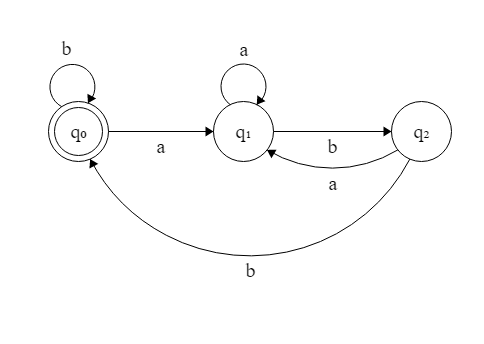
\includegraphics[scale=.75]{#4.png}
\item Trace the computation of $M$ that processes $babaab$.
\newline $q_0 \rightarrow q_1 \rightarrow q_2 \rightarrow q_1 \rightarrow q_1 \rightarrow q_2$
\item Give a regular expression for $L(M)$.
\newline $(b^*aa^*b(ab)^*)^*$
\item Give a regular expression for the language accepted if both
  $q_0$ and $q_1$ are accepting states.
  \newline $(b^*aa^*b(ab)^*b*aa*)^*$
\end{enumerate}

\item Define a DFA, $M$, that accepts the set of strings, $s$, over
  $\{a, b\}$ such that the substring $aa$ occurs at least twice in
  $s$. Draw the state 
  diagram for $M$. Give a regular expression for $L(M)$. 
  \newline 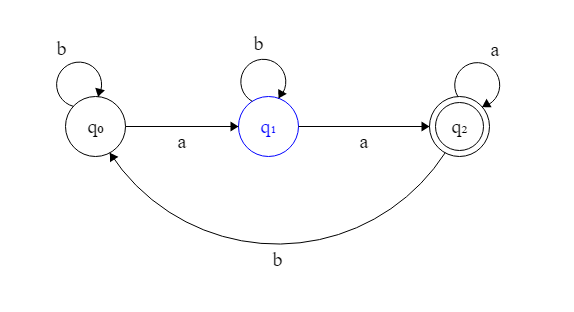
\includegraphics[scale=.75]{#5.png}

\item Define a DFA, $M$, that accepts the set of strings, $s$, over
  $\{a, b\}$ such that $s$ has an odd length or ends with $aaa$.
  Draw the state
  diagram for $M$. Give a regular expression for $L(M)$. 
  \newline 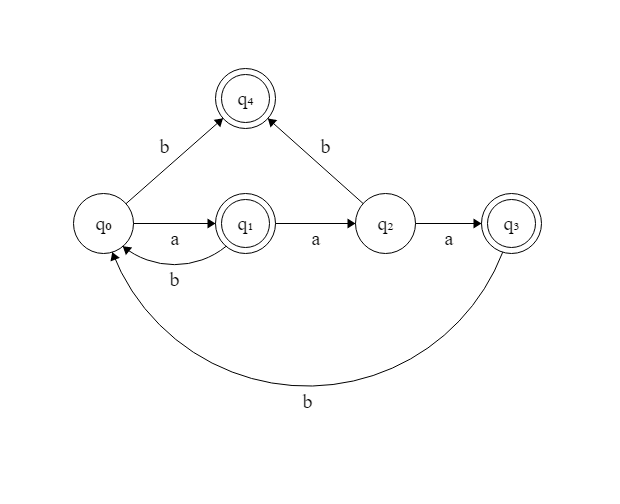
\includegraphics[scale=.75]{#6.png}

\end{enumerate}  
     
\end{document}


